\documentclass[platz]{tudphygp_eng}
\usepackage{tudphymd,mhchem}

\versuch{Diffusion}{DI}

\begin{document}
\maketitle

\section*{Task} 

The diffusion coefficient between \ce{NaCl}- solution and distilled water has to be determined by schlieren method after \textsc{Wiener}.

\medskip

Therefor following measuring tasks and evaluation procedures have to be carried out:

\begin{enumerate}
 \item Meassuring of $Y_{max}(t)$ for approximatly 8-20 time steps
 \item Plotting of the relation $t=f(Y_{max})$ in a linear manner (that means $t(Y_{max}^{-2})$-plot) and determination of the slope $m$ of this linear function
 \item Calculation of $D$ by using the slope $m$ of the $t(Y_{max}^{-2})$-plot and of the corresponding relation for $D$. The distance between cuvette and screen $E$, the length of the cuvette $x$ and the refracting indices $n_o$ (air), $n_1$ (\ce{NaCl}-solution) and $n_2$ (\ce{H2O}) have to be taken from this experimental guideline. 
\end{enumerate}

\section*{General information}

\begin{enumerate}
 \item At beginning: check, if all containers are cleaned and fixed in their locking position. The diffusion container do not have to be taken off from tripod during the whole time of experiment!
 \item After finishing of the experiments, all containers, as well as the diffusion container, have to be cleaned with distilled water. 
 \item Pay Attention during handling with glassware! The optical table is covered with crease for corrosion protection!
 \item The used light source is an He-Ne-laser, which emits coherent, parallel light with a wavelength of $\lambda= 632,8 ~ \mathrm{nm}$. 
 By using a rotatable glass rod (cylindrical lense) the focused laser spot has to be expanded to a line shape.\\
 \textbf{Attention:} The used laser has a safety class of IIb, that means the power is high enough for potential damaging your retina at direct incident of laser light into your eyes. Do not put reflecting items or even your eyes direct into the laser beam. Please use the provided laser protection glasses for adjustment of the experimental setup. The laser do not have to be operated without supervision.  
\end{enumerate}

\section*{Hints for generation of a sharp interface within the diffusion container}

Cuvette and reservoirs for solutions are shown schematically  in Fig.\ref{abb_aufbau}.

\begin{figure}[ht] 
 \centering 
 \label{abb_aufbau}
  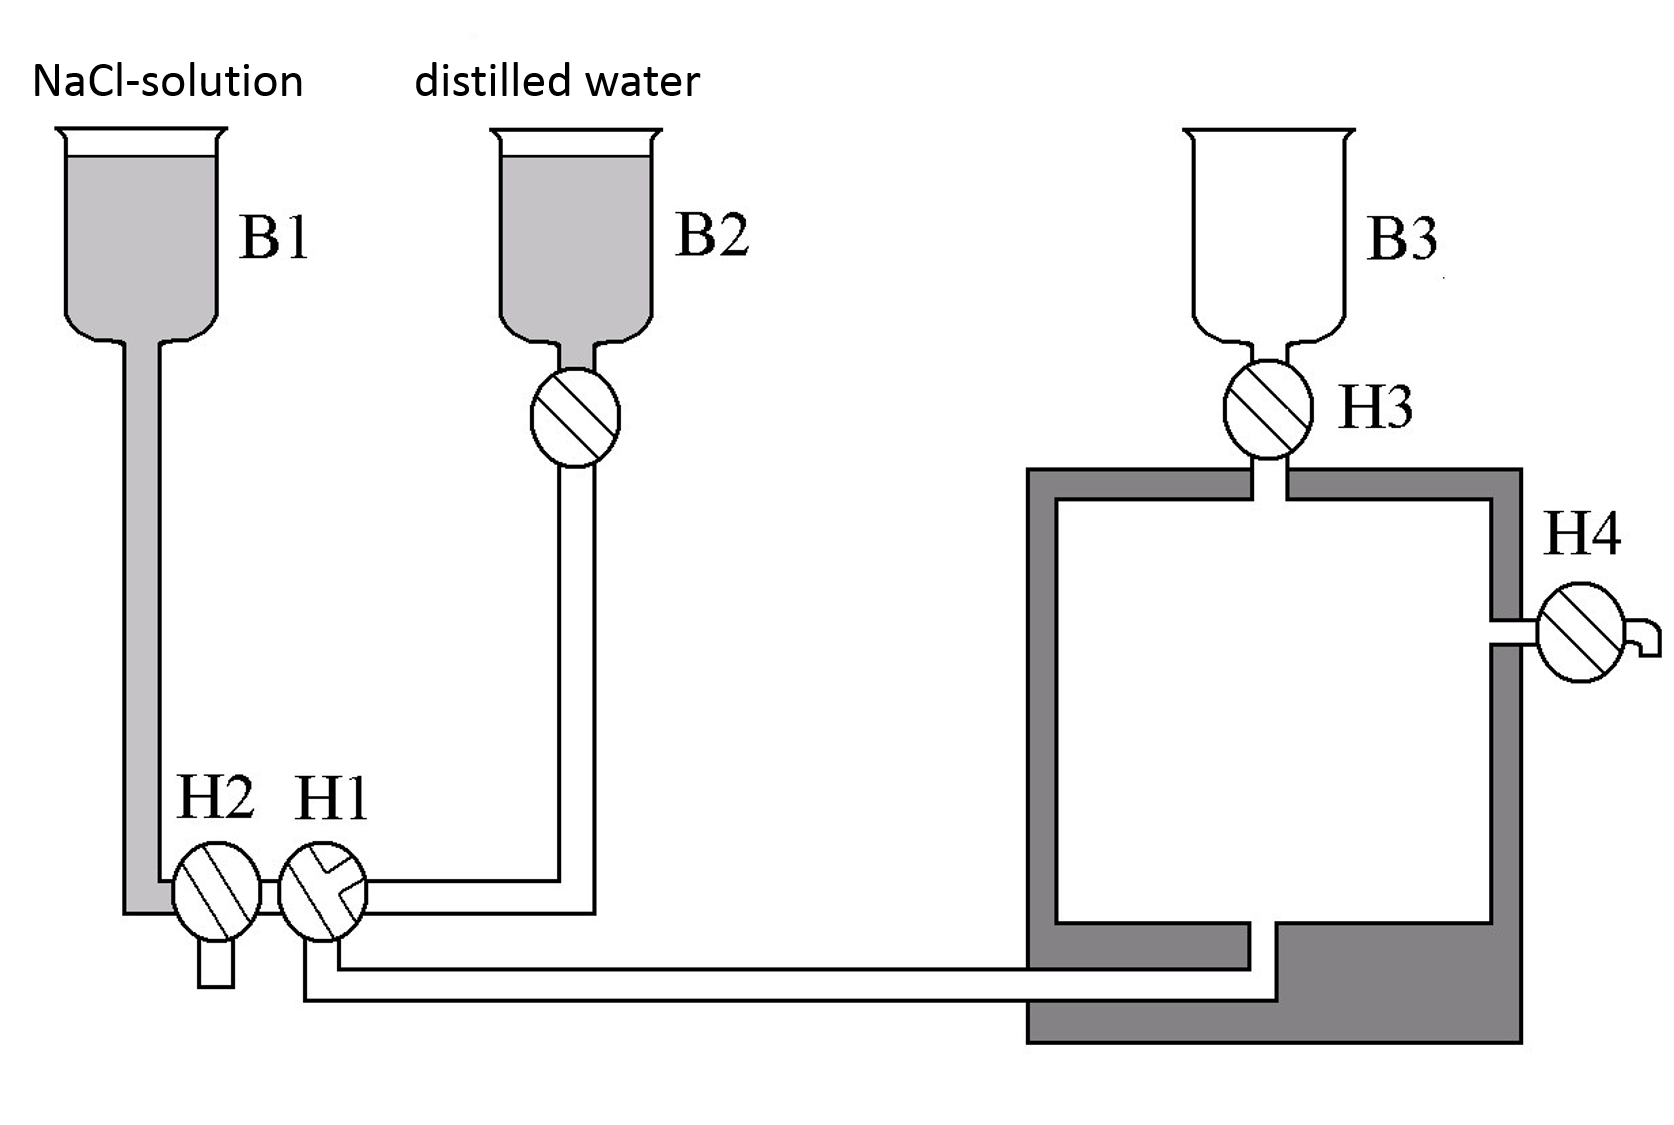
\includegraphics[width=10cm]{GP2-DI-kurz-aufbau_en.png}
 \centering 
 \caption{Schematic setup of diffusion cuvette and reservoirs}
\end{figure}

For the experiment following process steps are necessary:

\begin{enumerate}
 \item Filling up of the reservoirs B1 with \ce{NaCl}-solution and of B2 with distilled water. Make sure, that the valves H1 und H2 are closed. 
 \item Filling up the cuvette with distilled water from B2 to B3 until the distilled water level is just below the rising tube B3.\\
 \textbf{Attention:} You have to fill up very slowly for avoiding air bubbles in pipe and cuvette. Please consider the position of the three-way valve H1 as well of the valve H3 (open) and H4 (closed).
\item The setup have to be adjusted (by oriention of the laser and by rotatation of the cylindrical lens) so that laser light enters the cuvette in a small slit with a horizontal inclination of 45$°$. On the screen arranged behind the cuvette you have to build up an intensive and narrow projection of the strip. Afterwards fix a sheet of millimeter paper on it and draw in the strip base line by ruler and pencil. 
 \item Underlay the \ce{NaCl}-solution from B1 by slowly opening of the three-way valve H1. This process has to be continued until the level  of interface is a little bit higher than the pipe of valve H4.\\
 \textbf{Attention:} You have to fill up very slowly to avoid mixing effects of the interface. The level in rising tube B3 should rise only with slow velocity $< 1 ~ \frac{\mathrm{mm}}{\mathrm{s}}$!
\item The final sharp interface will be generated by slowly opening of H4 and slowly drain off the already mixed solution (approximately 1 drop per second). For this procedure H1 have to be closed and H3 have to be opened. 
A successful sharpening of the interface will be expressed by huge increasing $Y_{max}(t=0)=Y_0$.     
 \item H4 will be closed when reaching the maximum von $Y$, which is in the range of $20 \ldots 30 ~ \mathrm{cm}$ by careful preparation. The reached position $Y_{max}(t=0)=Y_0$ has to plot onto screen by fitting a tangent line parallel to the strip base line. The touching point of the tangent line and the curved laser strip marks the position of $Y_0$.
Afterwards in appropriative time steps further $Y_{max}$- values should be marked (for instance at reaching a diffusion time of $30\mathrm{s};1;2;3;5;7;9;11;15;20; \ldots \mathrm{min}$.
 
 \item Duration for the filling up procedure: $\approx ~ 45 ~ \mathrm{min}$
\end{enumerate}

\section*{ Technical and physical parameters}

For generation of \ce{NaCl}-solution $38~\mathrm{g}$ of \ce{NaCl} will bee solved in $200~\mathrm{cm}^3$ distilled water. This results in following concentration $c$ of the \ce{NaCl}-solution:

\begin{equation*}
 c = \frac{m_{\mathrm{NaCl}}}{m_{\mathrm{solution}}} \cdot 100 ~ \% = 16,00 ~ \%
\end{equation*}

Geometrical parameters of the cuvette:

\begin{itemize}
 \item Thickness of the glass plate: $(4,8~\pm~0,1) ~ \mathrm{mm}$
 \item Length $x$ of the cuvette:\\
 $\mbox{DI 1} \quad x = (13,5 ~\pm~ 0,2) ~ \mathrm{mm}$\\
 $\mbox{DI 2} \quad x = (12,84 ~\pm~ 0,06) \mathrm{mm}	$
\end{itemize}

Refractive index of air: $n_0 =1,00029$ \\
Refractive index \ce{NaCl}-solution: $n_1=1,586$ \\
Refractive index distilled water: $n_2=1,332$

\end{document}




